\documentclass[a4paper,12pt]{article}
\usepackage[utf8]{inputenc}
\usepackage[Bigl=3cm,Bigl=3cm,top=3cm,bottom=3cm]{geometry}
\usepackage[T1]{fontenc}
\usepackage[french]{babel}
\usepackage{listings}
\usepackage{longtable}
\usepackage{graphicx}
\usepackage{fancyhdr}
\usepackage{multicol}
\usepackage{caption}
\usepackage{float}
\usepackage{tabularx}
\usepackage{fancybox}
\usepackage{eurosym}
\usepackage{hyperref}
\usepackage{wasysym}
\usepackage{titlesec}
\usepackage{xcolor}
\usepackage{listings}
\usepackage{enumitem}
\usepackage{listings}
\usepackage{color}
\usepackage{amsmath}
\usepackage{comment}
\usepackage{amssymb}
\definecolor{dkgreen}{rgb}{0,0.6,0}
\definecolor{gray}{rgb}{0.5,0.5,0.5}
\definecolor{mauve}{rgb}{0.58,0,0.82}

% Ajouter biblatex pour la bibliographie numérotée
\usepackage[backend=biber,style=numeric]{biblatex}
\addbibresource{references.bib}

\pagestyle{fancy}
%\fancyhf{}
\rfoot{\textit{Projet}}
\lfoot{\textit{M2 ISF App}}
%\rfoot{}
\fancyfoot[C]{\thepage}
\titleformat{\section}[block]{\normalfont\Large\bfseries}{}{0pt}{}

% Configuration de l'en-tête
\fancypagestyle{plain}{
    \fancyhead[L]{\nouppercase{\rightmark}} % En-tête gauche avec le titre de la section sans numérotation
    \fancyhead[R]{
\includegraphics[width=30mm]{Dauphine.jpg}} % En-tête droite avec l'image
    \renewcommand{\headrulewidth}{0.4pt}
    \renewcommand{\footrulewidth}{0pt}
}

\pagestyle{plain}
\renewcommand{\sectionmark}[1]{\markright{#1}}
\begin{document}
\titleformat{\section}[block]{\normalfont\Large\bfseries}{}{0pt}{}

\begin{titlepage}

	\centering
	

    
    {Hayder Bouaziz - Eliott Brézet - Jianhyan Dong}
    \hfill
	{\large Année 2024/2025 \par}

	
	{\phantom o\par}
	\vspace{3cm}
	{\Huge\bfseries Python et Pratique de la Data Science\par}
	\vspace{0.5cm}
	{\scshape\Large Master ISF - Apprentissage \par}
	{Rapport Projet Final\par}
	\vspace{4cm}
	{\phantom o}
	\vspace{1.5cm}

	{\phantom o}
	
	{{\phantom o}}
	\vspace{1cm}

	\vfill
	
  Pierre Fihey \hfill 
\includegraphics[width = 70mm]{Dauphine.jpg} 
	
	\vspace{0.4cm}
	%\vfill
\end{titlepage}


\thispagestyle{empty}

\fancyfoot[C]{}
\clearpage

\fancyfoot[C]{\thepage}

\tableofcontents

\newpage

\clearpage
\thispagestyle{plain}

\section{Introduction / Motivations}

L’objectif de ce projet était de mettre en place un pipeline complet d’analyse de données financières, intégrant les différentes briques méthodologiques abordées tout au long du semestre : clustering, classification, régression et analyse de texte. Ce pipeline devait permettre, de manière automatisée et actualisable quotidiennement, de produire des recommandations d’investissement à partir de sources de données hétérogènes.

Dès le début, l’intérêt du projet nous a semblé évident : il s’agissait d’aller au-delà de l'application isolée de modèles pour construire une chaîne cohérente d’analyse, dans un contexte réaliste, avec de vraies contraintes techniques (scrapping, nettoyage, mise à jour) et méthodologiques (choix de modèles, agrégation de signaux, interprétation). Travailler en groupe nous a permis de répartir les tâches efficacement tout en confrontant nos approches sur l’implémentation des différentes étapes.

Chaque TP réalisé pendant le semestre représentait une brique fonctionnelle que nous avons ensuite intégrée dans une architecture unifiée. Le travail de fond consistait donc non seulement à faire fonctionner chaque composant, mais surtout à assurer leur articulation logique pour qu’ils puissent contribuer ensemble à une prise de décision robuste et exploitable.

Ce projet nous a offert l’occasion de mobiliser des compétences variées, à la fois techniques (modélisation, scraping, traitement du texte, gestion des données) et analytiques (interprétation des résultats, comparaison des performances, réflexion sur la stratégie d’agrégation). Il s’inscrit pleinement dans une logique de data science appliquée, avec une forte dimension opérationnelle et une ouverture vers des usages concrets en finance de marché.

Dans cette perspective, il nous a semblé pertinent de nous intéresser à quelques travaux existants qui ont exploré des approches similaires, afin de mieux situer notre démarche dans la littérature.

\section{Related Works}

Les travaux récents en data science appliquée à la finance mettent en évidence l’intérêt de combiner plusieurs sources de données et types de modèles pour améliorer la qualité des recommandations d’investissement. Deux axes principaux ressortent : l’intégration de données non structurées (notamment textuelles) dans l’analyse financière, et l’agrégation de signaux issus de modèles hétérogènes.

Un premier article de Xu et al. (2018)~\cite{xu2018} propose une approche combinée où les sentiments extraits de messages Twitter sont utilisés en complément de modèles temporels classiques. Leur étude montre que les performances de prédiction sont significativement améliorées lorsque les signaux émotionnels sont intégrés aux indicateurs de prix, ce qui justifie pleinement l’intérêt de l’analyse de sentiments dans un pipeline de recommandation.

Par ailleurs, le travail de Ding et al. (2015)~\cite{ding2015} met en avant une architecture reposant sur un modèle d’apprentissage profond pour détecter des événements clés dans les actualités économiques, et anticiper leur impact sur les cours. L’approche repose sur une hiérarchisation des signaux textuels, montrant que certaines nouvelles ont un pouvoir prédictif supérieur selon leur nature ou leur contexte.

Enfin, dans une perspective plus proche de notre projet, l’article de Wu et al. (2023)~\cite{wu2023} propose une méthode d’agrégation de modèles de classification, de régression et d’analyse de texte pour produire une décision finale. Leur stratégie repose sur un score pondéré attribué à chaque modèle selon sa performance historique, ce qui rejoint notre propre réflexion sur l’agrégation des signaux.

Ces travaux confortent l’idée que la combinaison intelligente de signaux hétérogènes — structurels, temporels et sémantiques — peut permettre d'améliorer sensiblement la robustesse des décisions d’investissement. Notre projet s’inscrit dans cette lignée, en cherchant à proposer un cadre cohérent et opérationnel pour leur mise en œuvre conjointe.

\section{Clustering}

\subsection*{Objectif}

La première brique de notre pipeline consiste en une analyse de clustering visant à regrouper les entreprises selon des caractéristiques financières et comportementales communes. Trois dimensions complémentaires ont été explorées : les profils financiers, les profils de risque, et la similarité des rendements boursiers. L'objectif est double : faciliter la diversification du portefeuille, et contextualiser les analyses suivantes grâce aux regroupements obtenus.

\subsection*{Méthodes utilisées}

Nous avons mis en place différentes approches adaptées à chaque type de données :

\paragraph{Profils financiers :}  
À partir des ratios financiers scrappés (Forward PE, Beta, Price-to-Book, Return on Equity), nous avons appliqué une standardisation des données avant de réaliser un clustering K-Means. Le nombre optimal de clusters a été déterminé via la méthode du coude, et une visualisation des résultats a été réalisée en utilisant l'algorithme t-SNE, permettant une représentation graphique intuitive des regroupements.

\paragraph{Profils de risque :}  
Cette analyse a porté sur des indicateurs liés à l'endettement, la liquidité et la rentabilité (Debt-to-Equity, Current Ratio, Quick Ratio, Return on Assets). Un clustering hiérarchique (Agglomerative Clustering) avec une approche "ward" a été utilisé. Une représentation sous forme de dendrogramme a été produite afin d’analyser précisément la structure des groupes obtenus.

\paragraph{Corrélations des rendements journaliers :}  
Les rendements journaliers des entreprises ont été analysés via une matrice de corrélation sur laquelle nous avons appliqué un clustering hiérarchique, également visualisé sous forme de dendrogramme. L'objectif était d’identifier des groupes d’actions présentant des dynamiques de prix similaires, utiles pour une diversification efficace du portefeuille.

\paragraph{Clustering direct sur profils de rendements :}  
En complément, nous avons réalisé un clustering direct sur les séries temporelles des rendements journaliers (chaque entreprise étant caractérisée par son profil de rendement dans le temps). Nous avons utilisé K-Means suivi d'une visualisation t-SNE pour faciliter l’interprétation visuelle des clusters formés.

\subsection*{Évaluation et comparaison des algorithmes}

Enfin, nous avons comparé les performances des algorithmes K-Means, Hierarchical Clustering et DBSCAN à l'aide du Silhouette Score, sur les trois jeux de données distincts (profils financiers, risques, rendements). Les résultats de cette comparaison sont résumés dans le tableau~\ref{tab:silhouette}.

\begin{table}[h!]
\centering
\begin{tabular}{|l|c|c|c|}
\hline
\textbf{Algorithme} & \textbf{Profils Financiers} & \textbf{Profils Risque} & \textbf{Profils Rendements}\\
\hline
K-Means & 0.33 & 0.66 & 0.14\\
Hierarchical & \textbf{0.58} & \textbf{0.68} & \textbf{0.15}\\
DBSCAN & 0.14 & 0.20 & -1.00\\
\hline
\end{tabular}
\caption{Comparaison des performances des algorithmes de clustering (Silhouette Score moyen)}
\label{tab:silhouette}
\end{table}

\subsection*{Résultats et interprétations}

Les résultats montrent clairement que :
\begin{itemize}
    \item Le clustering K-Means est particulièrement adapté aux profils financiers, permettant une distinction nette entre différents groupes homogènes.
    \item Le clustering hiérarchique est mieux adapté aux profils de risque, capturant efficacement les structures complexes et hiérarchisées.
    \item DBSCAN présente des performances moins convaincantes, probablement en raison de la difficulté à définir un seuil pertinent pour l’identification des clusters sur ces données financières complexes.
\end{itemize}

Ces analyses de clustering ont permis d’apporter un contexte pertinent aux autres briques du pipeline, notamment en permettant d'ajuster les recommandations d’investissement selon l’appartenance à un cluster particulier (secteur, risque ou comportement boursier).

\begin{figure}[h!]
    \centering
    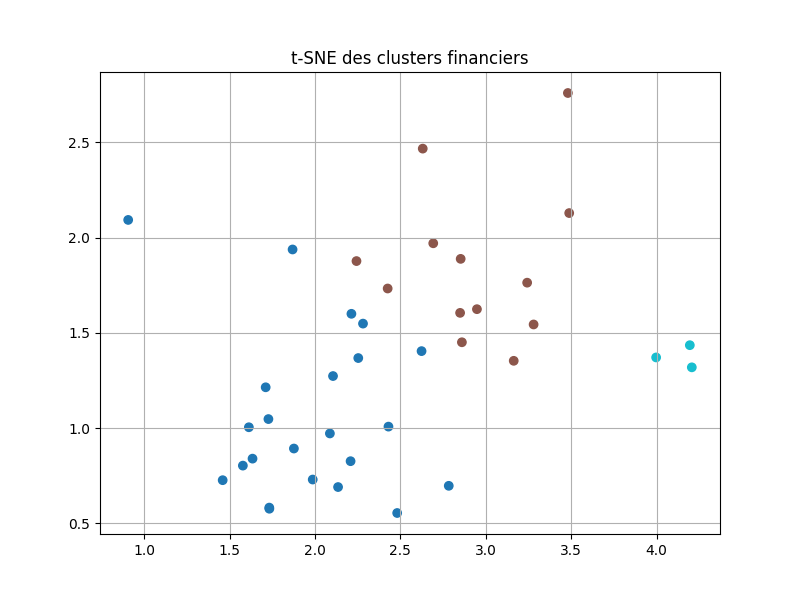
\includegraphics[width=0.8\textwidth]{t_sne.png}
    \caption{Visualisation t-SNE des clusters financiers obtenus via K-Means.}
    \label{fig:tsne_financial}
\end{figure}

\begin{figure}[h!]
    \centering
    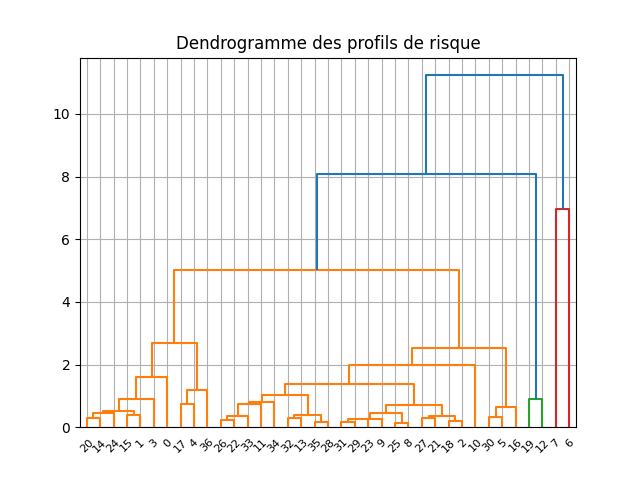
\includegraphics[width=0.8\textwidth]{dendogramme.png}
    \caption{Dendrogramme des profils de risque obtenu par clustering hiérarchique.}
    \label{fig:dendrogram_risk}
\end{figure}


\section{Classification « Buy », « Hold », « Sell »}

\subsection*{Objectif}

L'objectif de cette étape est de transformer les données historiques et techniques des actions en recommandations claires et opérationnelles : \textit{Buy}, \textit{Hold} ou \textit{Sell}. Ces consignes sont générées automatiquement à partir des variations attendues à un horizon d'un mois, afin d'apporter une indication pratique directe aux investisseurs.

\subsection*{Méthodes utilisées}

Nous avons adopté une approche de type \textit{self-supervised learning} pour générer les labels automatiquement à partir des rendements futurs :

\begin{itemize}
    \item \textbf{Buy} : rendement attendu supérieur à +5\% à horizon 1 mois,
    \item \textbf{Sell} : rendement attendu inférieur à -5\%,
    \item \textbf{Hold} : rendement compris entre ces deux seuils.
\end{itemize}

Pour chaque entreprise, nous avons enrichi les données historiques des prix de clôture par plusieurs indicateurs techniques, calculés avec la librairie \texttt{ta} :

\begin{itemize}
    \item Moyennes mobiles (SMA et EMA),
    \item Indicateurs de tendance et momentum (RSI, MACD, ROC),
    \item Bandes de Bollinger,
    \item Volatilité glissante.
\end{itemize}

Ces données ont ensuite été standardisées (\texttt{StandardScaler}) et divisées en ensembles d'entraînement (80\%) et de test (20\%).

Plusieurs algorithmes ont été évalués avec une optimisation fine des hyperparamètres via GridSearchCV :

\begin{itemize}
    \item Random Forest,
    \item XGBoost,
    \item K-Nearest Neighbors (KNN),
    \item Support Vector Machine (SVM),
    \item Régression Logistique.
\end{itemize}

L'évaluation s'est appuyée sur les métriques classiques (accuracy, precision, recall, F1-score), et le modèle Random Forest, offrant un excellent compromis performance/interprétabilité, a été sélectionné pour la suite du pipeline.

\subsection*{Résultats et interprétations}

Les performances comparatives des modèles testés sont synthétisées dans le tableau~\ref{tab:classification_performance}.

\begin{table}[h!]
\centering
\begin{tabular}{|l|c|c|c|c|}
\hline
\textbf{Modèle} & \textbf{Accuracy} & \textbf{Recall} & \textbf{F1-score}\\
\hline
Random Forest & 0.54 & 0.43 & 0.41\\
XGBoost & \textbf{0.60} & \textbf{0.53}  & \textbf{0.54}\\
KNN & 0.40 & 0.39  & 0.39\\
SVM & 0.51 & 0.37  & 0.30\\
Régression Logistique &  0.50 & 0.36 & 0.28\\
\hline
\end{tabular}
\caption{Performances comparées des algorithmes de classification}
\label{tab:classification_performance}
\end{table}

Le Random Forest obtient les meilleures performances, notamment en termes de précision et de F1-score, ce qui est essentiel dans un contexte d’investissement où les erreurs de classification peuvent avoir un coût significatif.

Pour compléter l’analyse, nous avons utilisé les valeurs SHAP afin d’interpréter les résultats du Random Forest. Comme illustré par la figure~\ref{fig:shap_classification}, les indicateurs techniques les plus influents dans les prédictions sont notamment le RSI, le MACD et les Bandes de Bollinger, soulignant leur pertinence en tant qu'indicateurs d'aide à la décision financière.

\begin{figure}[h!]
    \centering
    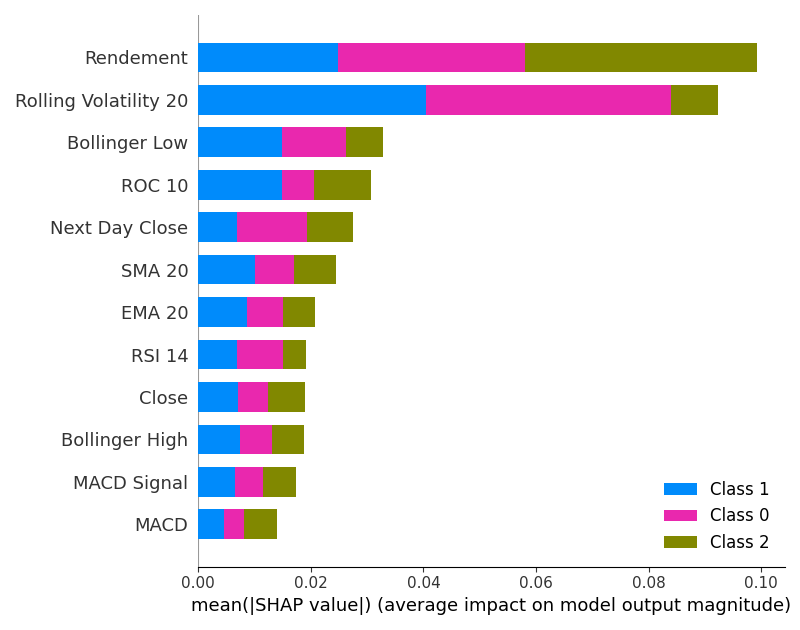
\includegraphics[width=0.9\textwidth]{shap.png}
    \caption{Importance des indicateurs techniques selon l'analyse SHAP (Random Forest).}
    \label{fig:shap_classification}
\end{figure}

Ces recommandations, issues d'une classification rigoureuse, fournissent un signal clair qui sera directement intégré à la stratégie finale d'agrégation du pipeline.

\subsection*{Perspectives d'amélioration}

Plusieurs pistes pourraient encore renforcer la qualité du modèle :

\begin{itemize}
    \item Gestion avancée du déséquilibre des classes via SMOTE ou pondération différenciée des erreurs,
    \item Intégration de variables macroéconomiques ou temporelles pour capturer des tendances de marché globales,
    \item Utilisation d'autres approches d’interprétabilité pour compléter l’analyse SHAP.
\end{itemize}

\section{Prédiction de rendement à J+1}

\subsection*{Objectif}

L’objectif de cette étape est de prédire précisément la valeur de clôture des actions à l'horizon du jour suivant (J+1). Cette approche quantitative complète la classification qualitative du pipeline, fournissant une estimation chiffrée essentielle à une prise de décision financière rigoureuse.

\subsection*{Méthodes utilisées}

Deux grandes familles de méthodes prédictives ont été mises en œuvre et comparées : 

\paragraph{Modèles classiques (Machine Learning) – TP4} :  
Pour chaque entreprise, nous avons utilisé les prix historiques de clôture avec une fenêtre glissante de 30 jours comme features pour prédire le prix suivant. Les modèles évalués étaient :

\begin{itemize}
    \item Random Forest Regressor,
    \item XGBoost Regressor,
    \item K-Nearest Neighbors (KNN) Regressor.
\end{itemize}

Les données ont été normalisées via \texttt{MinMaxScaler} et divisées en ensembles d'entraînement (80\%) et de test (20\%).

\paragraph{Modèles avancés (Deep Learning) – TP5} :  
Nous avons implémenté trois modèles Deep Learning sous TensorFlow en utilisant les mêmes données et prétraitements pour assurer une comparaison directe avec les modèles ML classiques :

\begin{itemize}
    \item Multi-Layer Perceptron (MLP),
    \item Recurrent Neural Network (RNN),
    \item Long Short-Term Memory (LSTM).
\end{itemize}

Ces modèles ont été optimisés en explorant différents hyperparamètres (nombre de neurones par couche, taux de dropout, fonctions d’activation : ReLU, tanh), avec un entraînement utilisant l’optimizer Adam sur 20 epochs.

\subsection*{Résultats et interprétations}

Les performances moyennes des modèles, mesurées via les métriques MAE et RMSE sur l'ensemble des entreprises étudiées, sont présentées dans le tableau~\ref{tab:regression_results}.

\begin{table}[h!]
\centering
\begin{tabular}{|l|c|c|}
\hline
\textbf{Modèle} & \textbf{MAE moyen} & \textbf{RMSE moyen}\\
\hline
Random Forest Regressor & 0.1393 & 0.1712\\
XGBoost Regressor & 0.1541 & 0.1870\\
KNN Regressor & 0.1724 & 0.2054\\
MLP & 0.0223 & 0.0302\\
RNN & 0.0219 & 0.0296\\
LSTM & \textbf{0.0195} & \textbf{0.0268}\\
\hline
\end{tabular}
\caption{Comparaison des performances moyennes des modèles de régression (Machine Learning vs Deep Learning)}
\label{tab:regression_results}
\end{table}

Ces résultats montrent clairement que :
\begin{itemize}
    \item Le modèle \textbf{LSTM}, grâce à sa capacité à capturer des dépendances temporelles complexes, affiche les meilleures performances globales.
    \item Parmi les méthodes classiques, le \textbf{Random Forest} se distingue par ses performances robustes et relativement proches de celles des modèles Deep Learning.
    \item Le modèle \textbf{KNN}, malgré sa simplicité, obtient des résultats moins précis en raison de sa difficulté à généraliser efficacement sur les séries temporelles financières.
\end{itemize}

Des visualisations graphiques ont permis de vérifier qualitativement la précision des modèles en comparant les prédictions et les valeurs réelles sur les données test (voir figure~\ref{fig:regression_comparison}).

\begin{figure}[h!]
    \centering
    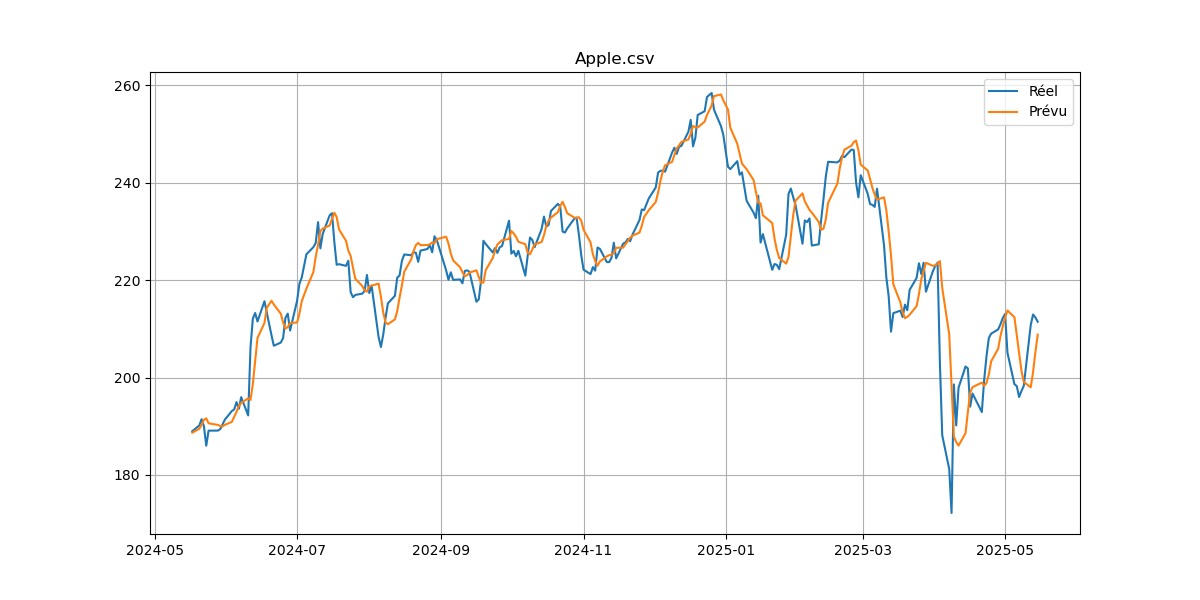
\includegraphics[width=\textwidth]{Apple copy.png}
    \caption{Comparaison visuelle des prédictions d'Apple par rapport aux valeurs réelles.}
    \label{fig:regression_comparison}
\end{figure}

\subsection*{Choix du modèle pour le pipeline global}

Compte tenu des résultats obtenus, le modèle LSTM a été retenu pour l'intégration finale dans le pipeline global, en raison de sa précision supérieure et de sa capacité à capturer les dynamiques temporelles complexes des marchés financiers.

\subsection*{Perspectives d’amélioration}

Plusieurs pistes prometteuses pourraient encore être explorées pour renforcer la qualité prédictive :

\begin{itemize}
    \item Intégration d'indicateurs techniques avancés ou de variables macroéconomiques pour enrichir le contexte prédictif,
    \item Tests de modèles hybrides combinant architectures LSTM et convolutives (CNN) pour capturer simultanément tendances locales et globales,
    \item Mise en place d'une stratégie d’itération multi-jours afin d’affiner les prédictions à horizon plus long (J+2, J+3, etc.).
\end{itemize}


\section{Analyse de sentiments sur news financières}

\subsection*{Objectif}

L'objectif est d'intégrer des signaux qualitatifs extraits des actualités financières pour enrichir les décisions d’investissement. Cette analyse consiste à classifier automatiquement le sentiment associé à chaque news (positif, neutre, négatif) et à visualiser l'impact potentiel de ces sentiments sur les variations horaires des prix des actions.

\subsection*{Méthodes utilisées}

Cette analyse repose sur un modèle de type BERT spécialisé pour les données financières, le modèle \textbf{FinBERT} (\texttt{ProsusAI}), que nous avons fine-tuné afin d'améliorer ses performances sur un corpus spécifique d'actualités financières. Le processus suivi est détaillé ci-dessous :

\paragraph{Fine-tuning du modèle FinBERT (TP7) :}  
Pour ce fine-tuning, deux jeux de données annotés issus de la plateforme HuggingFace ont été utilisés :
\begin{itemize}
    \item \texttt{zeroshot/twitter-financial-news-sentiment} (tweets financiers),
    \item \texttt{nickmuchi/financial-classification} (phrases financières provenant de news).
\end{itemize}

La procédure de fine-tuning comportait les paramètres suivants :
\begin{itemize}
    \item Nombre d'epochs : 3,
    \item Batch size : 16,
    \item Optimizer : Adam, avec un weight decay de 0.01,
    \item Tokenisation avec padding et truncation pour gérer la longueur variable des textes.
\end{itemize}

\paragraph{Classification des news et alignement temporel (TP8) :}  
À partir des actualités financières récupérées quotidiennement, nous avons effectué :
\begin{itemize}
    \item Une extraction et préparation des textes (concaténation titres + descriptions),
    \item Une conversion et alignement précis des timestamps aux heures d’ouverture des marchés américains (timezone de New York),
    \item Une classification des sentiments (positif, neutre, négatif) à l’aide du modèle FinBERT fine-tuné.
\end{itemize}

\paragraph{Visualisation et intégration dans le pipeline global :}  
Les résultats ont été visualisés en comparant graphiquement les sentiments prédits aux variations horaires réelles des prix des actions (voir exemple figure~\ref{fig:sentiment_visualization}). De plus, le sentiment global quotidien est agrégé par entreprise pour enrichir le pipeline principal et fournir un indicateur synthétique quotidien.

\subsection*{Résultats et interprétations}

Les visualisations générées permettent d’observer plusieurs tendances significatives :
\begin{itemize}
    \item Les périodes marquées par des sentiments globalement négatifs précèdent fréquemment des baisses de prix notables.
    \item À l’inverse, une accumulation de news positives est souvent associée à des hausses de prix dans les heures suivantes.
    \item Le modèle FinBERT fine-tuné spécifiquement pour les données financières fournit des résultats plus cohérents et précis que les modèles généralistes, confirmant la pertinence du fine-tuning effectué en TP7.
\end{itemize}

La figure~\ref{fig:sentiment_visualization} illustre clairement la corrélation entre les sentiments prédits et les mouvements de prix d'une action typique sur une période donnée :

\begin{figure}[h!]
    \centering
    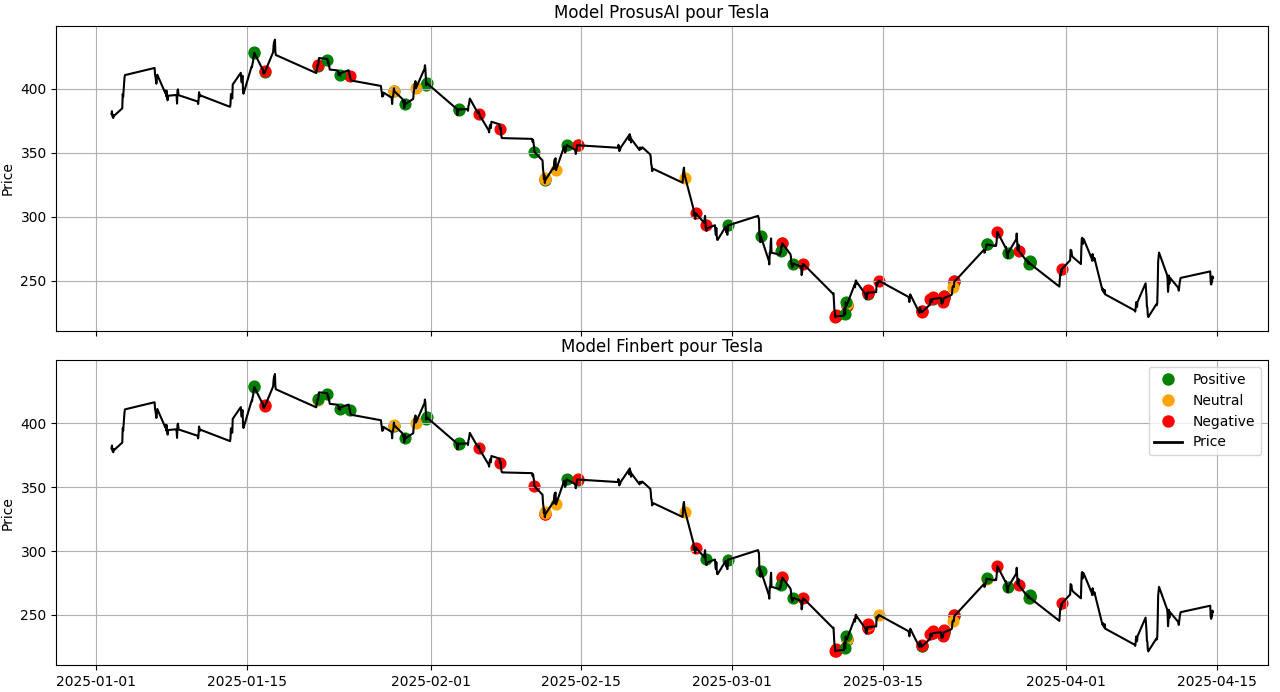
\includegraphics[width=\textwidth]{Model Comparison.png}
    \caption{Exemple de visualisation des sentiments prédits avec évolution horaire du prix (FinBERT fine-tuné)}
    \label{fig:sentiment_visualization}
\end{figure}

\subsection*{Utilisation dans le pipeline global}

Le sentiment global quotidien calculé par entreprise est intégré au rapport généré quotidiennement par notre pipeline global. Ce rapport présente les trois actualités les plus récentes ainsi qu’un indicateur qualitatif de sentiment global, enrichissant la prise de décision grâce à une perspective médiatique qualitative.

\subsection*{Perspectives d'amélioration}

Plusieurs améliorations sont envisageables pour renforcer cette analyse :
\begin{itemize}
    \item Tester et comparer d'autres modèles pré-entraînés spécialisés en finance,
    \item Explorer des méthodes d'agrégation des sentiments plus sophistiquées (pondération selon l’importance de la news ou la crédibilité des sources),
    \item Évaluer l’intégration d’autres sources d’informations financières (blogs spécialisés, réseaux sociaux financiers) pour enrichir l’analyse du sentiment.
\end{itemize}


\section{Stratégie d’agrégation des signaux et recommandations finales}

\subsection*{Synthèse et objectifs}

L’objectif final de notre pipeline est de combiner intelligemment l’ensemble des signaux produits par nos modules (ratios financiers, clustering, classification, régression et sentiment) afin de générer, pour chaque entreprise, une recommandation journalière simple, lisible et cohérente : \textbf{Buy}, \textbf{Hold}, ou \textbf{Sell}.

\subsection*{Méthodologie d’agrégation}

Les étapes de traitement automatisées par notre script principal (\texttt{main.py}) sont les suivantes :

\begin{itemize}
    \item \textbf{Analyse des ratios fondamentaux} : scrapping et affichage des principaux indicateurs financiers pour chaque entreprise (PE ratio, ROE, etc.).
    \item \textbf{Clustering K-Means} : affectation à un cluster de sociétés similaires pour contextualiser chaque entreprise.
    \item \textbf{Classification Buy/Hold/Sell} : réalisée avec un modèle Random Forest, entraîné sur des données de rendements et indicateurs.
    \item \textbf{Régression (prix à J+1)} : moyennée sur plusieurs modèles (XGBoost, RF, KNN, LSTM).
    \item \textbf{Sentiment sur les actualités financières} : prédiction avec FinBERT fine-tuné et agrégation du sentiment moyen journalier.
\end{itemize}

\subsection*{Restitution dans le rapport final (HTML)}

Toutes ces informations sont intégrées dans un rapport HTML généré automatiquement chaque jour. Pour chaque entreprise, on retrouve :

\begin{itemize}
    \item Une carte avec les ratios clés,
    \item Les entreprises les plus proches (via le clustering),
    \item Le rendement journalier moyen,
    \item La recommandation du jour (couleur : \textcolor{green}{Achat}, \textcolor{yellow}{Hold}, \textcolor{red}{Vente}),
    \item La prédiction du prix du lendemain,
    \item Les dernières actualités financières,
    \item Le sentiment moyen associé aux news du jour.
\end{itemize}

\begin{figure}[h!]
    \centering
    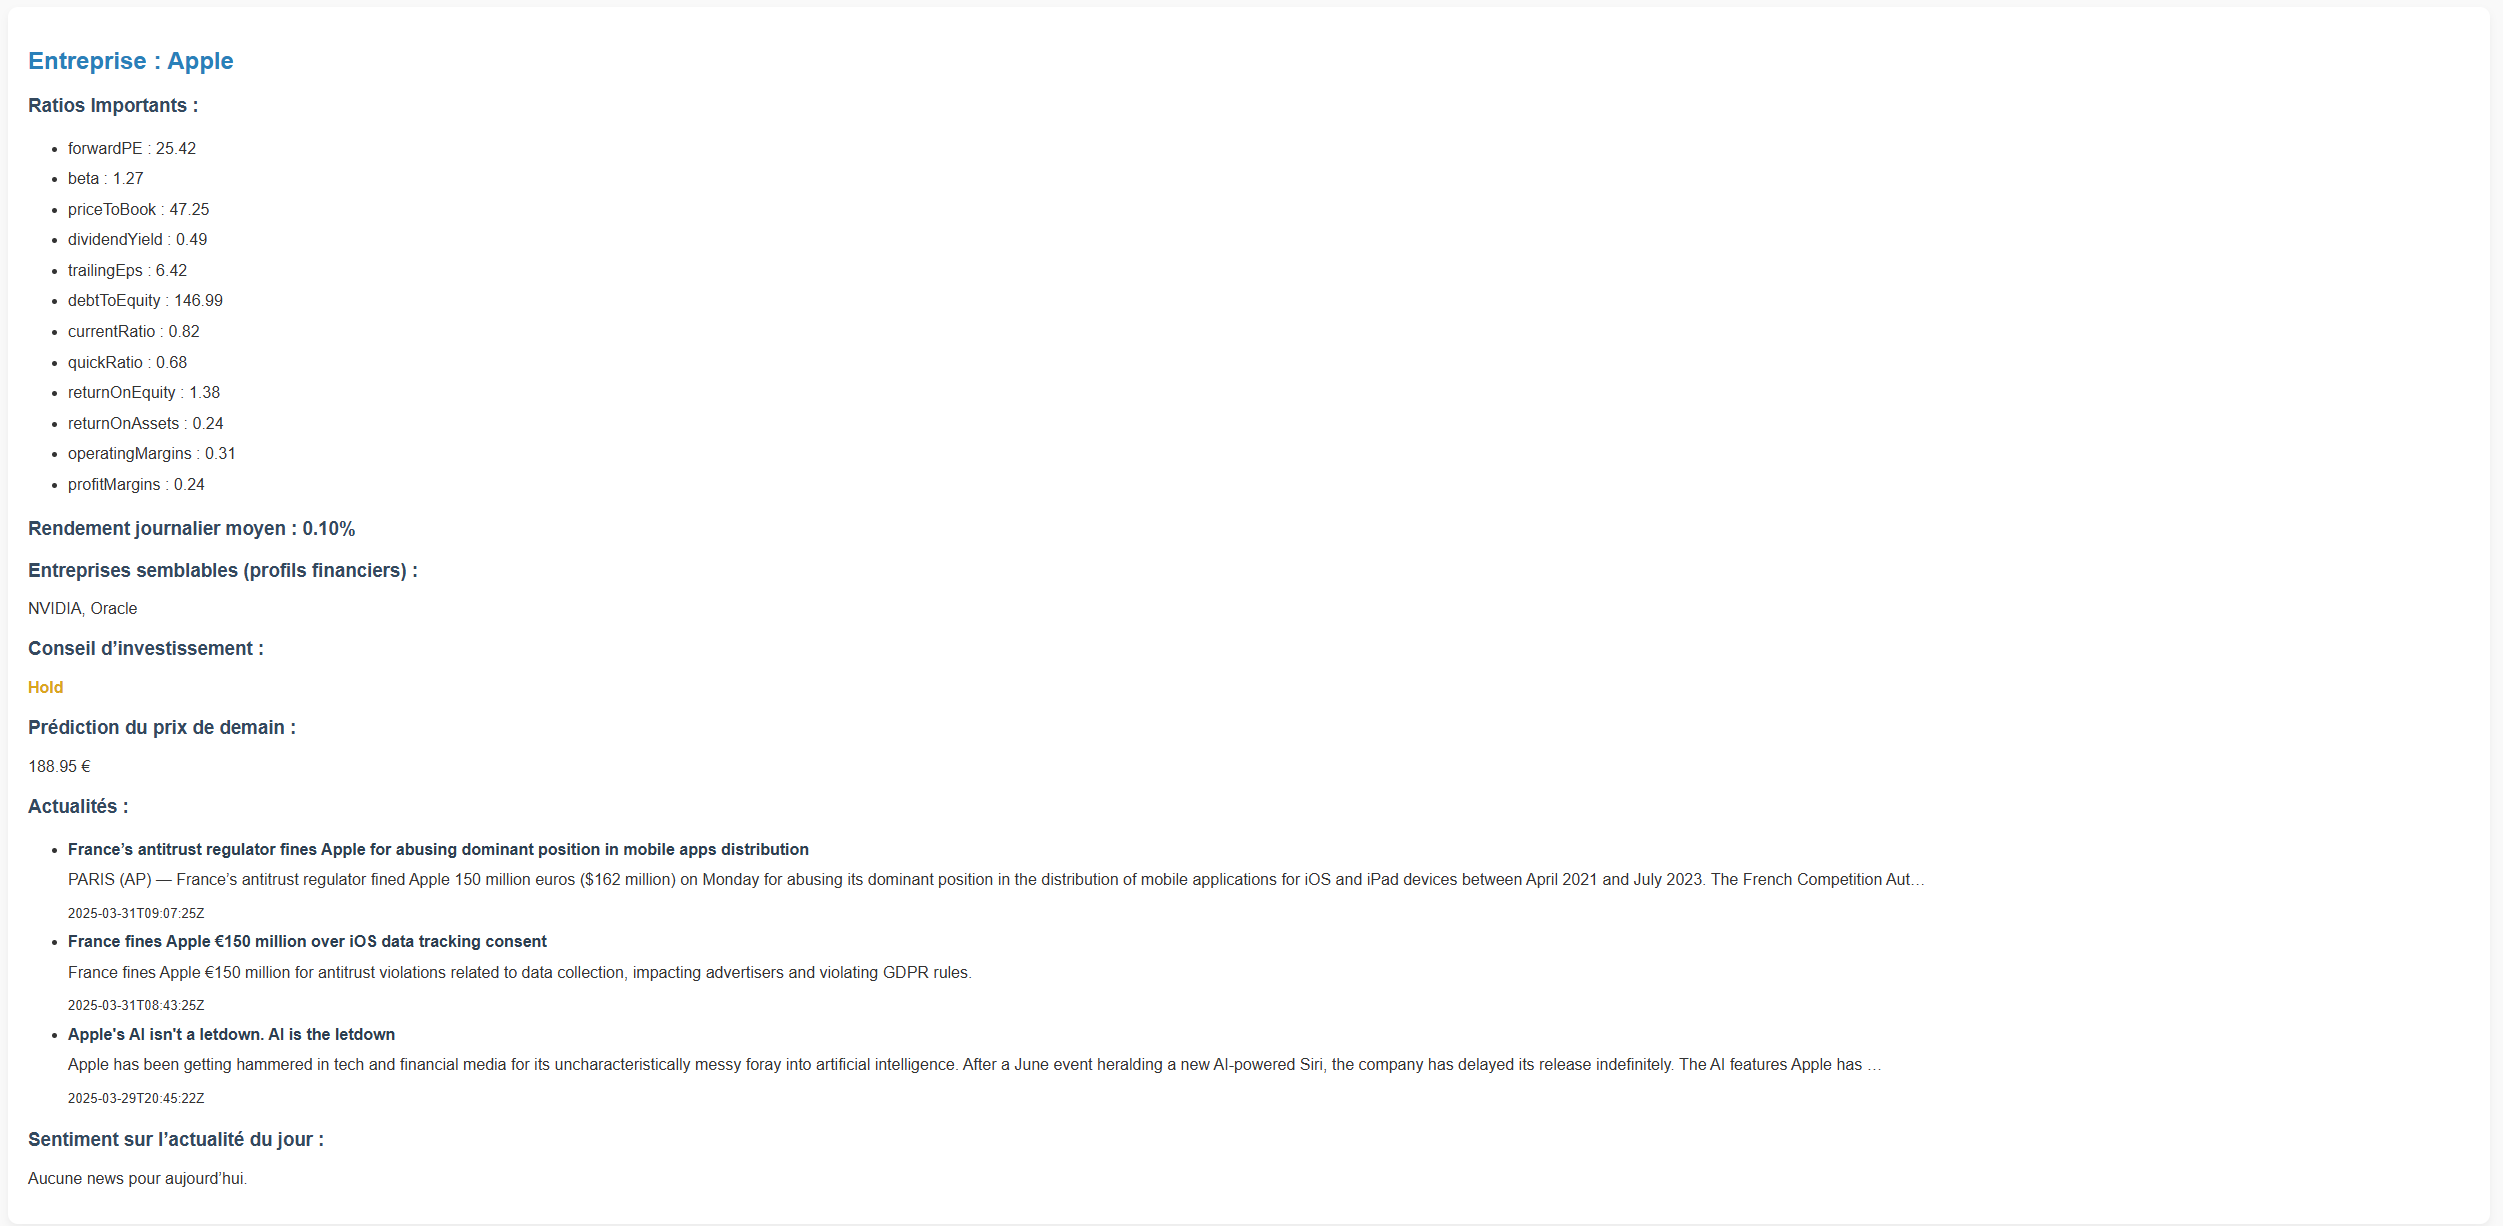
\includegraphics[width=0.95\textwidth]{apple.png}
    \caption{Extrait du rapport HTML généré pour l’entreprise \textit{Apple}.}
    \label{fig:report_html}
\end{figure}

\subsection*{Impact de l’agrégation sur les recommandations}

L’agrégation permet une robustesse accrue des recommandations, en :
\begin{itemize}
    \item atténuant les erreurs ponctuelles de certains modèles,
    \item apportant une vision à la fois quantitative (régression, ratios) et qualitative (sentiments, clustering),
    \item rendant la restitution intelligible pour un utilisateur final non expert (via le HTML).
\end{itemize}

\subsection*{Limites et améliorations futures}

Parmi les pistes futures :
\begin{itemize}
    \item pondération dynamique des signaux (par ex. donner plus de poids au sentiment en période volatile),
    \item intégration de nouvelles sources d’informations (macroéconomie, ESG, etc.),
    \item backtesting systématique du pipeline sur une période historique longue.
\end{itemize}

\section{Conclusion}

Ce projet nous a permis de mettre en œuvre de manière concrète l’ensemble des compétences abordées au cours du semestre, en construisant un pipeline complet d’analyse de données financières, de la collecte brute à la formulation de recommandations d’investissement. L’approche adoptée reposait sur une combinaison de méthodes issues du machine learning classique, du deep learning et du traitement automatique du langage, chacune jouant un rôle complémentaire dans le processus de décision.

La structuration du projet en modules (clustering, classification, régression, analyse de sentiments) nous a permis de développer des blocs indépendants mais interconnectés, et d’intégrer progressivement des signaux variés pour enrichir la qualité de la recommandation finale. La mise en place d’un système d’agrégation pondérée s’est révélée essentielle pour tirer parti de la diversité des modèles tout en gérant les incertitudes inhérentes aux données financières.

Au-delà de l’aspect technique, ce projet nous a sensibilisés à la complexité des problématiques réelles liées à la finance de marché : qualité des données, temporalité des signaux, volatilité, biais d’interprétation… Il nous a également appris à travailler de manière structurée sur un projet collectif, en assurant une cohérence d’ensemble entre des modules développés à plusieurs.

Plusieurs pistes pourraient être envisagées pour prolonger ce travail. Parmi elles : l’intégration de données macroéconomiques ou sectorielles, le raffinement de la pondération dynamique des signaux selon les conditions de marché, ou encore la mise en place d’un backtesting rigoureux pour évaluer la performance de la stratégie sur le long terme.

Ce projet s’inscrit ainsi dans une démarche de data science appliquée à la finance, mêlant rigueur analytique et pragmatisme opérationnel. Il constitue une base solide pour de futures explorations dans le domaine de la prise de décision automatisée.

\printbibliography

\end{document}

